\subsection{Fyzicka implementace}
Fyzická implementace definuje \textbf{datové struktury} pro základní logické objekty:

\begin{itemize}
\item \textbf{tabulky},
\item \textbf{indexy},
\item \textbf{materializované pohledy} (materialized views),
\item \textbf{rozdělení dat} (data partitioning) --  data s dlouhou historií. Fyzické rozdělení datových struktur a souboru na více částí.
\end{itemize}

Fyzická implementace tedy \textbf{řeší uložení dat na nejnižší úrovni databáze}.
 Na úrovni databáze můžeme ovlivnit výběr efektivnějšího plánu vykonávání dotazu případně \textbf{dobu vykonávání operací}.

\begin{itemize}
\item \textbf{ROWID} -- jedinečné číslo \textbf{označující záznam tabulky}.
\item Větší část teorie fyzického návrhu DB je platná pro libovolné SŘBD, dále se musíme řídit \textbf{doporučením výrobce}.
\item Každé SŘBD obsahuje specifickou reprezentaci tabulek a indexů:
\begin{itemize}
\item \textbf{CREATE TABLE} - vytvoření tabulky typu \textbf{halda} (Oracle), \textbf{shlukování záznamů} (SQL Server 2012).
\item \textbf{CREATE INDEX} - vytvoření\textbf{ B+-stromu}, kde každá položka odkazuje na ROWID záznamu v tabulce.
\end{itemize}
\end{itemize}

\subsection{Datové struktury}
Datové struktury \textbf{se skládají} buďto ze \textbf{stránek}, nebo z \textbf{uzlů} v případě stromové struktury. Jsou realizovány tak aby \textbf{operace} vyhledávání, vkládání, editace a mazání \textbf{byly co nejefektivnější}. 

Pro rychlé vyhledávání, které předchází i editaci a mazání je \textbf{nutné udržovat datovou strukturu setříděnou}. To však může zpomalit operaci vkládání (např. zařazením nového záznamu doprostřed tabulky musím posunout milion záznamů).
Základní datové struktury:

\begin{itemize}
\item \textbf{Blok} (alokační jednotka) -- je nejmenší jednotka, se kterou SŘBD manipuluje při zápisu a čtení dat z disku (obvykle 4KB nebo 8KB).
\item \textbf{Stránka} -- nejmenší jednotka s kterou pracuje správce paměti. \texttt{Stranka.velikost = X * Blok.velikost} (je-li velikost bloku = 4KB je odpovídá velikost stránky násobkům 4KB).
\item \textbf{Datový soubor} -- fyzický prostor na disku s daty.
\end{itemize}


\subsection{Typy tabulek}
\subsubsection{Heap Table}
\begin{itemize}
\item Implicitní pro \texttt{CREATE TABLE} (v MSSQL), záznamy nejsou nijak uspořádány.
\item \textbf{Stránkové perzistentní pole} s velikostí \textbf{bloku} nejčastěji \textbf{8kB}.
\item Záznamy pouze \textbf{označovány jako smazané}, pro fyzické smazání slouží speciální operace \textbf{shrinking}.
\item Při vkládání záznam uložen na \textbf{první volnou pozici v tabulce} nebo na \textbf{konec pole}.
\item Složitost operací: neefektivní vyhledávání $O(n)$, velmi \textbf{efektivní vkládání} $O(1)$ i \textbf{využití místa}.
\end{itemize}
\subsubsection{Shlukování záznamů (Data Clustering)}
\begin{itemize}
\item Záznamy v \textbf{datovém souboru jsou seřazeny podle zvoleného klíče}, pro implementaci nejčastěji využita nějaká \textbf{varianta B-stromu}.
\item Listové uzly stromu (bloky) obsahují \textbf{kromě klíče i další záznamy} tabulky.
\item Používá se všude, kde potřebujeme \textbf{získat i hodnoty ostatních atributů} (kromě klíče - např. \texttt{SELECT} neklíčových atributů).
\item \textbf{Zhoršený výkon} \texttt{INSERT} (data se musí zatřizovat).
\item \textbf{Oracle:} Index Organized Table (IOT), \textbf{SQL Server:} Clustered Index.
\end{itemize}

\subsubsection{Hašovaná tabulka (Hash Table)}
\begin{itemize}
\item Záznamy se stejnou hashovanou hodnou jsou uloženy ve stejném nebo velmi blízkém bloku.
\item Trochu \textbf{plýtvá místem}.
\item Musíme znát předem velikost záznamů (alespoň přibližně).
\end{itemize}

\subsubsection{Materializované pohled (Materialized views)}
\begin{itemize}
\item Uložené \textbf{výsledky dotazů}, které bývají často v DB vyhodnocovány.
\item Jde spíše o \textbf{fragment} z \textbf{tabulky} či několika tabulek.
\end{itemize}

\subsection{Indexy}
Indexové soubory slouží k \textbf{seřazení tabulky podle jiných atributů než je samotná tabulka defaultně seřazená}. Index je tedy vázaný ke konkrétní tabulce a konkrétnímu atributu podle kterého data řadí. Index umožňuje \textbf{rychlé vyhledávání} dle klíče, \textbf{ROWID pak odkazuje na kompletní záznam v heap tabulce}. \texttt{CREATE [BITMAP] INDEX login ON Student;}. 
\begin{itemize}
\item \textbf{Primární index (PRIMARY)} -- automatický index, který se váže k primárnímu klíči, zajišťuje jedinečnost údajů.
\item \textbf{Unikátní index (UNIQUE)} -- stejně jako primární index zajišťuje jedinečnost údajů v atributu, ale neváže se pouze ke klíči.
\item \textbf{Vedlejší index (INDEX)} -- klasické index popsány níže.
\item \textbf{Fulltextový index} -- používá se pro optimalizaci fulltextového vyhledávání v daném sloupci.
\end{itemize}

\subsubsection{Bitmapový index}
\textbf{Odpovídá na všechny možné hodnoty daného atributu}. Jde o tabulku jedniček a nul, kde řádky reprezentují záznamy v indexované tabulce a sloupce hodnoty indexovaného atributu. Jednička pak znamená true, že záznam má hodnotu danou sloupcem. \textbf{Vyplatí se}, pokud se používají logické operátory (\texttt{AND}, \texttt{OR}, \texttt{XOR}) \textbf{nad několika bitmapovými indexy atributů}.

\begin{figure}[H]
	\centering
	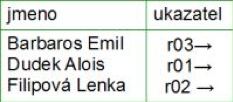
\includegraphics[width=0.3\textwidth]{assets/index_classic.png}
	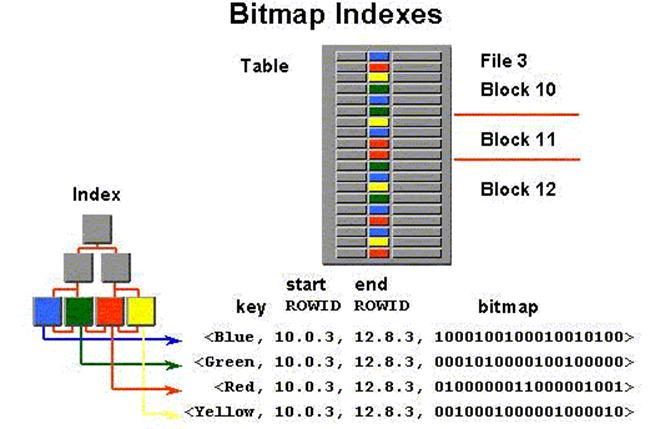
\includegraphics[width=0.65\textwidth]{assets/index_bitmap.jpg}
\end{figure}

\subsubsection{Shlukovaný index (Cluster Index)}
Pokud se pro dvě tabulky často používá operace spojeni (JOIN) pro jeden atribut. V tomto případě diskový blok obsahuje záznam z řídicí tabulky a zároveň i závislé záznamy. (v normalnim připadě obsahuje diskovy blok pouze zaznamy jedne tabulky).

\subsubsection{Kandidáti na index}
\begin{itemize}
\item \textbf{Primární} klíče a \textbf{cizí} klíče.
\item Pokud je index používán pro nalezení malého počtu záznamů.
\item Pokud index pokryje jeden nebo více častých dotazů.
\item Atributy často se vyskytující v konstrukci \texttt{WHERE}.
\end{itemize}

\subsection{Vykonávání dotazu}
\textbf{Ovlivnění času vykonávání dotazu} - parametrizované dotazy, hromadné operace, nastavení transakcí. Na úrovni DB můžeme ovlivnit výběr efektivnějšího plánu vykonávání dotazu, případně dobu vykonávání operací -> \textbf{fyzický návrh DB}. Identifikujeme \textbf{4 fáze vykonávání dotazu}:

\begin{enumerate}
	\item \textbf{Převod dotazu do interní formy}
	\begin{itemize}
		\item Převod původního dotazu do zvolené \textbf{interní formy}.
		\item \textbf{Eliminujeme syntaxi jazyka dotazu} (např. SQL).
		\item Zpracování pohledů, které probíhá v této fázi, znamená, že \textbf{nahradíme pohled jeho definicí} (materializované pohledy -- fragmenty/výsledky dotazů).
		\item Interní forma je nejčastěji \textbf{nějaký druh dotazovacího strom}u (angl. query tree).
	\end{itemize}
	\item \textbf{Převod do kanonické formy}
	\begin{itemize}
		\item V této fázi optimalizátor provádí celou řadu \textbf{optimalizací}.
		\item Převodem do kanonické formy dochází k \textbf{odstranění} různých povrchních \textbf{rozdílů} a především nalezení \textbf{efektivnějšího} \textbf{tvaru} než nabízel původní dotaz.
		\item \textbf{Optimalizátor} – transformační pravidla (převádí výraz na ekvivalentní). Fáze transformace/přepsání dotazu (query rewite). Dotaz tedy není ve skutečnosti vykonán přesně tak, jak byl zadán! 
	\end{itemize}
	\item \textbf{Výběr nízkoúrovňových procedur}
	\begin{itemize}
		\item V této fázi se optimalizátor rozhoduje jak bude transformovaný dotaz vykonán.
		\item Nyní optimalizátor uvažuje: \textbf{existenci indexů}, \textbf{distribuci hodnot}, \textbf{shlukování uložených dat}.
	\end{itemize}
	\item \textbf{Vygenerování plánů dotazu a výběr nejlevnějšího plánu}
	\begin{itemize}
		\item Cena procedury je závislá na aktuální \textbf{mohutnosti vstupních relací} a na mohutnosti \textbf{mezivýsledků jednotlivých procedur}.
		\item Odhad velikosti mezivýsledků je však často problematický jelikož velmi ovlivňuje cenu operace, jedná se o jeden z \textbf{nejřešenějších problémů}.
		\item Z množiny dotazovacích plánů pak \textbf{optimalizátor} vybírá ten \textbf{nejlepší}, tedy \textbf{nejlevnější}.
	\end{itemize}
\end{enumerate}

\subsection{Ladění dotazů}
\begin{itemize}
	\item Po vybrání nejlevnějšího plánu je \textbf{dotaz proveden} a uživateli vrácen výsledek.
	\item \textbf{Plán} lze v SŘBD většinou \textbf{zobrazit} - operace jako průchod tabulkou, přístup k indexu, třídění spojení atd. To lze využít pro \textbf{odladění dotazu} - např. uvidíme, že musíme použít index na neindexovaný atribut.
	\item Dvěma či více \textbf{různými dotazy} je možno obdržet \textbf{stejná data}. 
	\item \textbf{Rychlost} různých dotazů ovšem\textbf{ nemusí být stejná }i přesto, že vracejí stejná data.
	\item Snažíme dosáhnout \textbf{maximálního} \textbf{výkonu} se \textbf{stávajícími prostředky}.
	\item Plán vykonávání dotazu vybírá \textbf{optimalizátor}.
	\item Snažíme se vytvořit dotaz, který\textbf{ bude načítat z úložiště pouze to, co potřebuje}.
\end{itemize}

\subsubsection{Přístupy k ladění}
\begin{itemize}
\item \textbf{Proaktivní} -- Analyzujeme fyzický návrh a provádíme změny k lepšímu fungování.
\item \textbf{Reaktivní} -- Reagujeme na problém.
\end{itemize}

\subsubsection{Ladění výkonu SŘBD}
\begin{itemize}
	\item \textbf{HW} -- RAID, RAM, CPU (Poslení možnost, je to drahé, efektivnější je \textbf{vyladit fyzický návrh}).
	\item \textbf{Parametry SŘBD} -- Velikosti \textbf{cache}, maximum zámků, atd. Nutné optimalizovat na určité použití.
	\item \textbf{ORM} -- Minimum SQL příkazů a objemu přenášených dat. Úroveň izolace transakce.
\end{itemize}